\title{Extrapolating expected accuracies for multi-class classification}
\author{Charles Zheng, Rakesh Achanta and Yuval Benjamini}
\date{\today}

\documentclass[12pt]{article} 

% packages with special commands
\usepackage{amssymb, amsmath}
\usepackage{epsfig}
\usepackage{array}
\usepackage{ifthen}
\usepackage{color}
\usepackage{fancyhdr}
\usepackage{graphicx}
\usepackage{mathtools}
\usepackage{csquotes}
\usepackage{multirow}
\usepackage{xcolor}
\usepackage{chngcntr}
\usepackage{apptools}
\AtAppendix{\counterwithin{lemma}{section}}

\newcommand\crule[3][black]{\textcolor{#1}{\rule{#2}{#3}}}


\definecolor{grey}{rgb}{0.5,0.5,0.5}
\definecolor{color1}{RGB}{128,13,13}
\definecolor{color2}{RGB}{70,128,13}
\definecolor{color3}{RGB}{13,128,128}
\definecolor{color4}{RGB}{70,13,128}

\begin{document}
\maketitle

\newcommand{\tr}{\text{tr}}
\newcommand{\E}{\textbf{E}}
\newcommand{\diag}{\text{diag}}
\newcommand{\argmax}{\text{argmax}}
\newcommand{\Cov}{\text{Cov}}
\newcommand{\Var}{\text{Var}}
\newcommand{\argmin}{\text{argmin}}
\newcommand{\Vol}{\text{Vol}}
\newcommand{\comm}[1]{}
\newcommand{\indep}{\rotatebox[origin=c]{90}{$\models$}}
\newcommand{\Cor}{\text{Cor}}
\newtheorem{theorem}{Theorem}[section]
\newtheorem{proposition}{Proposition}[section]
\newtheorem{corollary}{Corollary}[theorem]
\newtheorem{lemma}{Lemma}[section]
\newcommand{\bZ}{\boldsymbol{Z}}
\newcommand{\bz}{\boldsymbol{z}}
\newcommand{\bx}{\boldsymbol{x}}
\newcommand{\bX}{\boldsymbol{X}}


\begin{abstract}
The difficulty of multi-class classification generally increases with
the number of classes.  Using data from a subset of the classes, can
we predict how well a classifier will scale with an increased number
of classes?  Under the assumption that the classes are sampled
exchangeably, and under the assumption that the classifier is
generative (e.g. QDA or Naive Bayes), we show that the expected
accuracy when the classifier is trained on $k$ classes is the $k-1$st
moment of a \emph{conditional accuracy distribution}, which can be
estimated from data.  This provides the theoretical foundation for
performance extrapolation based on pseudolikelihood, unbiased
estimation, and high-dimensional asymptotics.  We investigate the
robustness of our methods to non-generative classifiers in simulations
and one optical character recognition example.
\end{abstract}

\section{Introduction}
A computer that can use sensory information to automatically
 distinguish between multiple scenarios has increasingly many applications
 in modern life. Examples include detecting the speaker from his voice patterns, 
identifying the author from her written text, or labeling the object 
category from its image. All these examples can be described as multi-class classification problems:
the computer observes an input $x$, and uses the classifier function $f$ to guess
the label $y$ from a discrete set $\mathcal{Y}$ of possible labels. 
In all applications described above, the space of potential labels is practically infinite.
But in any particular experiment, the number of different labels $k$ used would be finite.
A natural question, then, is how does chabging the number of 
possible labels affect classification accuracy. 

More technically, we consider a sequence of classification
problems on finite label subsets
$\mathcal{S}_1 \subset \cdots \subset \mathcal{S}_K \subset \mathcal{Y}$,
where in the $i$-th problem, one constructs the classification rule
$f^{(i)}:\mathcal{X} \to \mathcal{S}_i$.  Supposing that $(X, Y)$ have
a joint distribution, define the misclassification error for the
$i$-th problem as
\[
\text{Err}^{(i)} = \Pr[f^{(i)}(X) \neq Y|Y \in \mathcal{S}_i].
\]
The problem of \emph{performance extrapolation} is the following: using data
from only $\mathcal{S}_k$, can one predict the misclassification error
 on the larger label set $\mathcal{S}_K$, with $K> k$?
Note that unlike other
extrapolations from a smaller sample to a larger population, 
the classification problem becomes harder as the number of distractor classes
increases. 

Accurate answers to this 
problem are not only of theoretical interest, but also have practical implications:
\begin{itemize} 
\item Example 1: A researcher develops a classifier for the purpose of labelling
images in 10,000 classes. However, for a pilot study, her resources are sufficient to 
tag only a smaller subset of these classes, perhaps 100. Can she estimate how well the algorithm 
work on the full set of classes based on an initial "pilot" subsample of class labels?
\item Example 2: A neuroscientist is interested in how well the brain activity 
in various regions of the brain can discriminate between different classes of stimuli.
Kay et al. [1] obtained fMRI brain scans which record how a single
subject's visual cortex responds to natural images. They wanted to know how 
well the brain signals could discriminate between different images. For a set of 1750
photographs, they constructed a classifier which
achieved over 0.75 accuracy of classification. Based on
exponential extrapolation, they estimate that it would take on the
order of $10^{9.5}$ classes before the accuracy of the model drops
below 0.10!  A theory of performance extrapolation could be useful for
the purpose of making such extrapolations in a more principled way.
\item The stories just described can be viewed as a metaphor for typical
paradigm of machine learning research, where academic researchers,
working under limited resources, develop novel algorithms and apply
them to relatively small-scale datasets. Those same algorithms may
then be adopted by companies and applied to much larger datasets with
many more classes. In this scenario, it would be convenient if one
could simply assume that performance on the smaller-scale
classification problems was highly representative of performance on
larger-scale problems. 
\end{itemize}

Previous works have shown that generalizing from a small set of classes 
to a larger one is not straightforward. In a paper titled ``What
does classifying more than 10,000 Image Categories Tell Us,'' Deng and
co-authors compared the performance of four different classifiers on
three different scales: a small-scale (1,000-class) problem,
medium-scale (7,404-class) problem, and large-scale (10,184-class)
problem (all from ImageNet.)  They found that while the
nearest-neighbor classifier outperformed the support vector machine
classifier (SVM) in the small and medium scale, the ranking switched
in the large scale, where the SVM classifier outperformed
nearest-neighbor.  As they write in their conclusion, ``we cannot
always rely on experiments on small datasets to predict performance at
large scale.'' Theory for performance
extrapolation may therefore reveal models with bad scaling properties in the
pilot stages of development.

Our primary goal in this paper is to formulate this question, and
identify scenarios where answers are possible. 
The most important condition is that the smaller problem would be 
representative of the larger one. For simplicity, we
assume that in both $\mathcal{S}_K$ and $\mathcal{S}_k$ are iid samples
from a population (or distribution) of labels. (Other sampling 
mechanisms would require some modification). 
The condition of i.i.d. sampling ensures that the
separability of random subsets of $\mathcal{Y}$ can be inferred by
looking at the empirical distributions in $\mathcal{S}_k$, and
therefore that some estimate of the achievable accuracy on
$\mathcal{S}_K$ can be obtained.

Furthermore, we restrict our analysis to a restricted set of classifiers,
\emph{marginal classifiers}, which train a separate model separately for each class. 
This convenient property allows us to
characterize the accuracy of the classifier by selectively
conditioning on one class at a time.  In section \ref{sec:extrapolation}, we use this
technique to reveal that the expected risk for classifying on the
label set $\mathcal{Y}_k$, for all $k$, is governed by a function
called the \emph{conditional risk} depends on the true distribution
and the classifier.  As long as one can recover the conditional risk
function $\bar{K}(u)$, one can compute the average risk for any number
of classes. 
  In section 5, we
empirically study the performance curves of classifiers on sequences
of classification tasks.  Since marginal classifiers only comprise a
minority of the classifiers used in practice, we applied our methods
to a variety of generative and non-generative classifiers in
simulations and in one OCR dataset.  Our methods have varying success
on generative and non-generative classifiers, but seem to work badly
for neural networks.

[[Move to Discussion:]]
In non-marginal classifiers, the classification rule has
a joint dependence on the entire set of classes, and cannot be
analyzed by conditioning on individual classes.
\newline

\noindent\emph{Our contribution.}

To our knowledge, we are the first to formalize the problem of
prediction extrapolation.  We develop a general theory for prediction
extrapolation under \emph{general class priors} and under bounded cost
functions.  In addition, we investigate the special case of zero-one
loss under uniform priors: we develop a pseudolikelihood-based
estimation approach for this special case, and evaluate its
performance in real data examples.

\subsection{Background: multi-class classification}

In this section we review the key terminology for multi-class
classification and discuss examples of problems and algorithms which
we will use throughout the paper to serve as concrete examples.  We
assume some degree of familiarity with statistical learning: however,
this section can probably be skipped by the expert.  Meanwhile, those
new to the field might be aided by having a good introduction to the
subject at hand, such as (Hastie et al, ESL) or (?? other book.)

While a \emph{binary classification} problem generally refers to a
class with two labels, $\mathcal{Y} = \{0, 1\}$, problems with three
or more classes are called \emph{multi-class classification} problems.
The most famous dataset for illustrating a multi-class classification
problem is Fisher's iris data (Fisher 1936), where the classification
task is to assign a flower to one of three iris species based on four
features: the lengths and widths of the sepals and the lengths and
widths of the petals.

In classification problems, it is assumed that each observation
belongs exclusively to a single class.  In contrast,
in \emph{multi-label} classification, each observation can belong to
multiple classes at the same time, or none at all.  We do not address
multi-label classification in this paper: however, we remark that any
multi-label classification problem can be recoded as a single-label
classification problem [find a reference so we don't have to explain
this.]

The performance of a classification rule on a problem is evaluated by
specifying a \emph{cost function.}  If the true class is $y$, but the
classifier outputs $y'$, the severity of this misclassification is
quantified by $C(y', y)$.  The most common cost function
is \emph{zero-one loss}: the cost is zero for correct classifications,
and the cost is one for all incorrect classifications, i.e. $C(y', y)
= \delta_{y}(y').$
% do we need to explain dirac delta?

One setting where alternative cost functions are used is when there
exists \emph{hierarchical structure} of the label sets.  For example,
in image recognition, the label ``golden retriever'' may be a member
of the class ``dog,'' which is in itself another label.  If we work
under the single-label framework, then a picture of a golden retriever
might be considered to have the true class of ``golden retriever.''
While labelling the picture as ``dog'' would be semantically correct,
we might prefer the more specific label.  But while on a technical
level we may consider ``dog'' to be the incorrect label for the
picture, we would not want to overly penalize the assignment of
``dog'' to the picture.  Therefore, in hierarchichal problems it is
often appropriate to use a cost function which is reflective of
the \emph{semantic distance} between two labels, rather than the
strict zero-one loss.

In our terminology, a \emph{classification model} is an algorithm
which learns a \emph{classification rule} from \emph{training data}.
Examples of multi-class classification models include $k$-nearest
neighbors, multinomial logistic regression, linear discriminant
analysis (LDA), quadratic discriminant analysis (QDA), decision trees,
and random forests, as well as the two `divide and conquer'
approaches, one-vs-one (OVO) and one-vs-all (OVA) (Friedman et al,
2008.)

The \emph{generalization risk} is the expected cost over the
population of label-feature pairs.  Given \emph{test data} sampled
from the population, it is possible to obtain an unbiased estimate of
the risk fof a classification rule.

% semantic distance is not explained

%The hierarchy of labels is often represented by a tree $T$, where the
%vertices $V$ are the set of labels, and the edges indicate
%superclass-subclass relationships.  One of the earlier examples is
%Chakrabarti (1998), who classified online texts into topic taxonomies.
%One of the taxonomies, reprinted from their paper, is shown in
%Figure \ref{fig:chakra}.
% sometimes the classes are only the leaves, and sometimes all nodes are classes

%\begin{figure}[h]
%\centering
%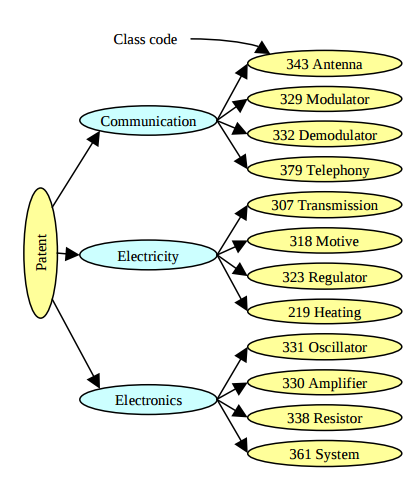
\includegraphics[scale = 0.4]{chakrabarti_1998.png}
%\caption{A topic taxonomy reprinted from Chakrabarti (1998)}\label{fig:chakra}
%\end{figure}

%Cost functions for hierarchical class function are commonly derived
%from graph distances induced by the tree $T$.  For example, one might
%define $C(y', y)$ to be the \emph{graph distance} between $y$ and
%$y'$--that is, the minimal number of edges in the graph for any path
%between $y$ and $y'$.

%[examples of multi-class classifiers? LDA, QDA, OVA, OVO?]

\section{Framework}\label{sec:formulation}

\subsection{Problem Formulation}

This section lays out the basic framework which is necessary to
\emph{formulate} the problem.  However, in the rest of the paper, we
will also adopt some additional assumptions in order to solve the
problem we pose in this section.

Let $\mathcal{Y}$ be a collection of labels and $\mathcal{X}$ be a
space of feature vectors.  For each label $y \in \mathcal{Y}$, there
exists a distribution $F_y$ supported on $\mathcal{X}$.  Also suppose
that there exists a \emph{cost function} $C(\hat{y}, y)$ which
measures the cost of incorrectly labelling an instance as $\hat{y}$
when the correct label is $y$.  Further suppose that $0 \leq C(y, y')
< \infty$ and $C(y, y)=0$ for all $y, y' \in \mathcal{Y}$.  (Recall
that in practice, the cost function is specified by the user to
reflect the needs of the application.)

A \emph{classification task} consists of a subset of labels,
$\mathcal{S} \subset \mathcal{Y}$, and a prior distribution $\pi$ over
the label subset.  Write $\mathcal{S}=\{y_1,\hdots, y_k\}$, where $k$
is the number of classes.  A \emph{classification rule} for the task
consists of a function $f$ which maps feature vectors
$x \in \mathcal{X}$ to labels in $\mathcal{S}$:
\[
f: \mathcal{X} \to \mathcal{S}.
\]
The classification task defines the \emph{risk} of a classification
rule.  Under the classification task, a label $y$ is drawn from the
distribution $\pi$.  Then, we draw $x \sim F_y$.  The label assigned
by the classification rule is $\hat{y} = f(x)$.  The \emph{loss}
incurred is $C(\hat{y}, y)$.  The \emph{risk} of the classification
rule is the expected loss under the class distribution $\pi$:
\[
\text{Risk}(f) = \E_\pi[C(\hat{y}, y)] = \int_\mathcal{S} d \pi(y) \int_{\mathcal{X}} C(f(x), y) dF_y(x).
\]

For label $y \in \mathcal{Y}$, define a sample of size $r$ as a
sequence of i.i.d. observations $X_1,\hdots, X_r \sim F_y$.
A sample can either be represented as a vector of points, or as
an \emph{empirical distribution} $\hat{F}_y$
\[\hat{F}_y = \frac{1}{r}\sum_{i=1}^r \delta_{x_i^{(y)}}.\]
Let $\Pi_{y, r}$ denote the sampling distribution of $\hat{F}_y$.

In the literature, the term \emph{classifier} is used ambiguously to
refer to either what we call the \emph{classification model} or
the \emph{classification rule.}  Here, we take a \emph{classification
model} $\mathcal{F}$ to mean an algorithm or procedure for producing
classification rules given an empirical distributions $\hat{F}_y$ for
each $y \in \mathcal{S}$, and a vector of prior probabilities $\pi$.
The model maps a distribution $G$ and a vector $\pi$ to a
classification rule $f$ (Figure \ref{fig:classification_rule}.)
Within this paper, we use the word \emph{classifier} as a shorthand
for \emph{classification model} when there is no danger of ambiguity.

We suppose that the \emph{training set}
$\{\hat{F}_y\}_{y \in \mathcal{S}}$ consists of samples of size
$r_{train}$ for each $y \in \mathcal{S}$
(Figure \ref{fig:training_set}.) Additionally, we assume that one has
access to a \emph{test set} of size $r_{test}$.  Notationally, we
always represent the training set samples for each class as empirical
distributions $\hat{F}_y$, while the test set samples are written as
vectors $(X^{(y)}_1,\hdots, X^{(y)}_{r_{test}})$.

\begin{figure}[h]
\centering
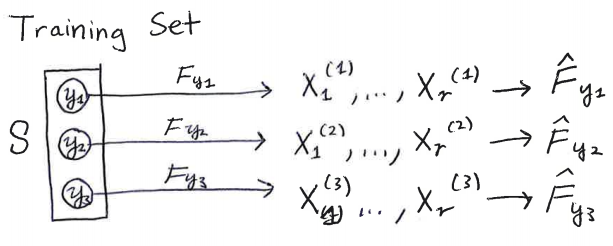
\includegraphics[scale = 0.4]{extrapolation_figures/training_set.png}
\caption{Training set}\label{fig:training_set}
\end{figure}

\begin{figure}[h]
\centering
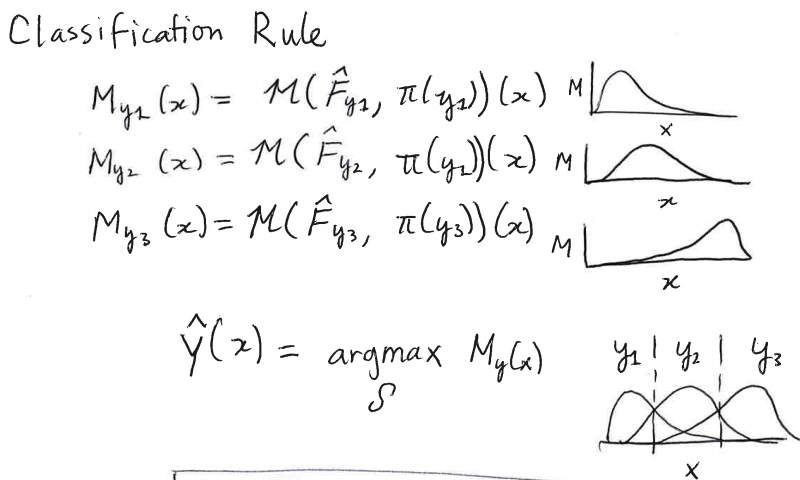
\includegraphics[scale = 0.4]{extrapolation_figures/classification_rule.png}
\caption{Classification rule}\label{fig:classification_rule}
\end{figure}

\begin{figure}[h]
\centering
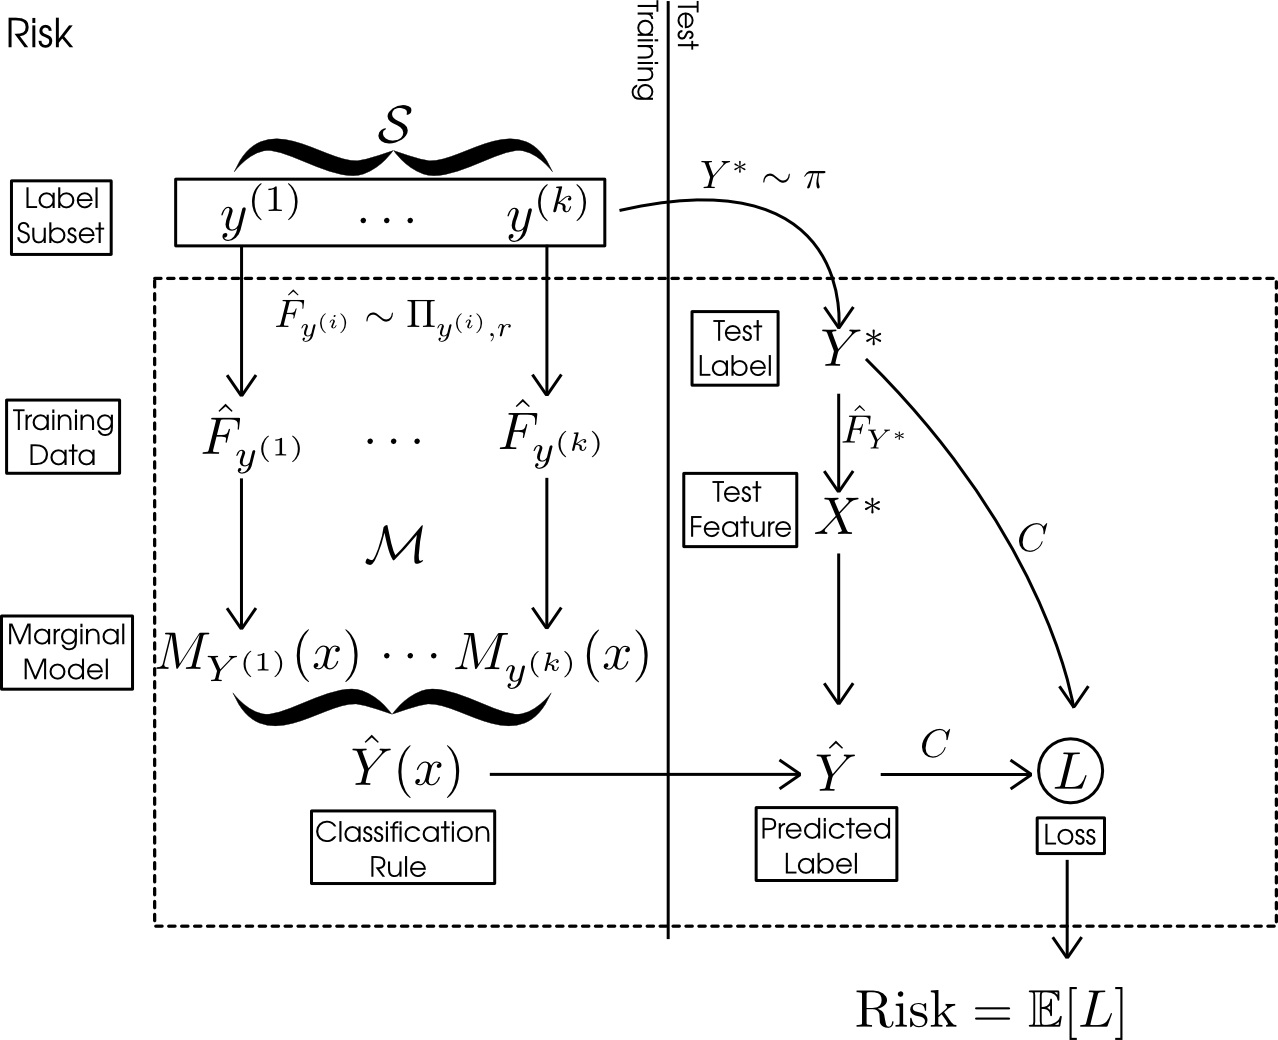
\includegraphics[scale = 0.4]{extrapolation_figures/risk.png}
\caption{Classification risk}\label{fig:risk}
\end{figure}

The $r$-repeat \emph{risk} of the classification model $\mathcal{F}$
is the expected risk of a classification rule $\hat{f} =
\mathcal{F}(\hat{F}_{y_1},\hdots, \hat{F}_{y_k})$ for the
classification task, $\hat{F}_y \sim \Pi_{y, r}$.  That is,
\[
\text{Risk}_r(\mathcal{F}; \pi) =
\int \text{Risk}(\mathcal{F}(\{\hat{F}_y\}_{y \in \mathcal{S}};
\pi)) \prod_{y \in \mathcal{S}} d\Pi_{y, r}(\hat{F}_y).
\]
Figure \ref{fig:risk} illustrates the variables involved in defining
the risk.

The problem of \emph{performance extrapolation} is as follows.
Suppose we have two classification tasks: the $i$th classification
task is specified by label subset $\mathcal{S}_i$, prior distribution
$\pi_i$.  We observe data from the first classification task
consisting of a dataset consisting of a training samples of size
$r_{train}$ per class, plus an independent test samples of size
$r_{test}$ per class.  The goal is to estimate the $r_{train}$-sample
risk of a $\mathcal{F}$ on the second classification task,
$\text{Risk}_{r_{train}}(\mathcal{F}; \pi_2)$.

\subsection{Additional assumptions}

In order to obtain a tractable solution to the problem of performance
extrapolation, we make a number of special assumptions on the nature
of the classification tasks, and the classifiers themselves, which
make the problem much easier.

Firstly, we assume that the label space $\mathcal{Y}$ is a continuum:
in fact, that $\mathcal{Y}$ is a subset of $d$-dimensional Euclidean
space. Note this is not such a strong assumption as it might seem,
since cases where there are $k$ discrete labels can be equivalently
formulated as continous models where the the continuum can be
partitioned into $k$ equivalence classes, and in which the cost
between two label $y, y'$ is a function only of their equivalence
classes.

We work with bounded cost functions, since such an assumption
simplifies the theory, and because unbounded cost functions can be
analyzed by taking a limit of bounded approximations.  Furthermore,
without loss of generality, we can assume that
\[
\sup_{y, y'\in \mathcal{Y}} C(y, y') \leq 1.
\]

With regards to the classification tasks, (i) we assume that there
exists some prior density $\pi_0$ over $\mathcal{Y}$, and that (ii)
the label subsets $\mathcal{S}_i = \{y^{(1,i)}, \hdots, y^{(k_i,i)}\}$
are obtained by iid samples with replacement from the density $\nu$.
We pause to remark on these assumptions.
\begin{itemize}
\item[i.]
The assumption of a prior density, when combined with the assumption
that $\mathcal{Y}$ is a continuum, implies that the probability of any
particular $y \in \mathcal{Y}$ is zero.  Therefore, this assumption
would seem to violate most applications of classification, where the
labels come from a discrete distribution.  However, any discrete
classification problem can be recoded as an equivalent continuous
classification problem.  Note that any discrete space $\mathcal{Y}$
can be expanded to a continuous space $\tilde{\mathcal{Y}}$ by means
of augmenting the label $y$ with an uninformative auxillary variable
$u \in [0,1]$.  By defining the cost function $\tilde{C}((y, u), (y',
u')) = C(y, y')$ and prior distribution $\tilde{\pi}_0 = \pi \times U$
where $U$ is the uniform distribution, we obtain an equivalent
classification problem which satisfies our assumptions.
\item[ii.(a.)]
We allow the sampling distribution of classes in the label subset to
differ from the prior probabilities, because $\pi_0$ reflects the
population distribution of $Y$ while $\nu$ reflects the mechanism
used to pick classes for the label subset.  In experimental settings,
$\nu$ is under the control of the experimenter, so it need not be
chosen to be identical to $\pi_0$.
\item[ii.(b.)]
Note that here we assumed that the label subsets $\mathcal{S}_1$ and
$\mathcal{S}_2$ are independent: as a consequence of (i), this means
that they are disjoint with probability one.  An alternative
assumption would be that $\mathcal{S}_1 \subset
\mathcal{S}_2$ with $\mathcal{S}_1$ being a subsample of
$\mathcal{S}_2$: this assumption can also be addressed, as we will
discuss later.
\end{itemize}

Now recall that the prior probabilities $\pi_i$ for each
classification task are free for the user to define, unlike the
population distribution $\pi_0$ of class labels which is assumed to
have an objective existence.  Since the subsampled or `small-scale'
classification tasks (with label subsets $\mathcal{S}_i$) are
presumably intended to approximate the `full' classification problem
(with the label set $\mathcal{Y}$), and since the prior in the full
problem is $\pi_0$, a sensible choice would be to choose
\[
\pi_i(y) = \frac{\pi_0(y)}{\sum_{y' \in \mathcal{S}_i} \pi_0(y')}.
\]
as the prior for the $i$th classification task.  As it turns out, such
a prior assignment also simplifies the theory, so we will assume that
$\pi_i$ is defined according to the above.

We make some rather strong assumptions with regards to the
classifiers.  The classifier $\mathcal{F}$ produces classification
rules $f$ which depend on \emph{marginal scoring rules}, $m_y$ for $y
\in \mathcal{S}$.  Each marginal scoring rule $m_i$ is a mapping
\[
m_y: \mathcal{X} \to \mathbb{R}.
\]
The classification rule chooses the class with the highest marginal score,
\[
f(x) = \text{argmax}_{y \in \mathcal{S}} m_y(x).
\]
The marginal scoring rules $m_i$, in turn, are generated by a marginal
model $\mathcal{M}$.  The marginal model converts empirical
distributions $\hat{F}$ over $\mathcal{X}$, and an (empirical) prior
class probability, into a marginal scoring function $m: \mathcal{X}
\times \mathbb{R} \to \mathbb{R}$.  For example, one could take 
\[m(x,p) = \log(p) + \log(\hat{f}(x)).\]
where $\hat{f}$ is a density estimate obtained from
$\hat{F}$.  We call such a classification model $\mathcal{F}$ a
\emph{marginal classifier}, and such marginal classifiers are
completely specified by the marginal model $\mathcal{M}.$

Quadratic discriminant analysis and Naive Bayes are two examples of
marginal classification models.
%\footnote{For QDA, the classification function is
%  given by
%\[
%\mathcal{Q}_{QDA}(\hat{F}, y) = -(y - \mu(\hat{F}))^T \Sigma(\hat{F})^{-1} (y-\mu(\hat{F})) - \log\det(\Sigma(\hat{F})),
%\]
%where $\mu(F) = \int y dF(y)$ and $\Sigma(F) = \int (y-\mu(F))(y-\mu(F))^T dF(y)$.
%In Naive Bayes, the classification function is
%\[
%\mathcal{Q}_{NB}(\hat{F},  y) = \sum_{i=1}^n \log \hat{f}_i(y_i),
%\]
%where $\hat{f}_i$ is a density estimate for the $i$-th component of
%$\hat{F}$.}.
The \emph{marginal} property allows us to prove strong results about
the accuracy of the classifier under i.i.d. sampling
assumption, as we see in Section [].

\subsection{Definition of average risk}\label{sec:average_risk}

Since the classification tasks are randomly generated, the $r$-repeat
risk becomes a \emph{random variable} which depends on the random
label subset $\mathcal{S}$.

Therefore, define the $k$-class, $r$-repeat \emph{average risk} of
classifier $\mathcal{F}$ with prior weights $\pi$ as
\[
\text{AvRisk}_{k, r}(\mathcal{F}; \pi) = \E[\text{Risk}_k(\mathcal{F}); \pi)]
\]
where the expectation is taken over the distribution of $\mathcal{S} =
(Y^{(1)},\hdots, Y^{(k)})$ when $Y^{(i)} \stackrel{iid}{\sim} \nu$.

As we can see from Figure \ref{fig:average_risk}, the average risk is obtained by averaging
over four randomizations:
\begin{enumerate}
\item[A1.] Drawing the label subset $\mathcal{S}$.
\item[A2.] Drawing the training dataset.
\item[A3.] Drawing $Y^*$ from $\mathcal{S}$ according to $\pi$.
\item[A4.] Drawing $X^*$ from $F_{X^*}$.
\end{enumerate}

For the sake of developing a better intuition of the average risk, it
is helpful to define a random variable called the \emph{loss}, which
is the cost incurred by a single test instance.  The loss is
determined by quantities from all four randomization steps: the label
subset $\mathcal{S} = \{Y^{(1)},\hdots, Y^{(k)}\}$, the training samples
$\hat{F}_{Y^{(1)}},\hdots, \hat{F}_{Y^{(k)}}$, and the test point $(X^*, Y^*)$.
Formally, we write
\[
L = C(\mathcal{F}(\{\hat{F}_y\}_{y \in \mathcal{S}}; \pi)(X^*), Y^*).
\]
Now note that the $k$-class, $r$-repeat average risk is the expected loss,
\begin{equation}\label{eq:avrisk_EL}
\text{AvRisk}_{k, r, \nu}(\mathcal{F}) = \E[L] = \E[C(\mathcal{F}(\{\hat{F}_y\}_{y \in \mathcal{S}}; \pi)(X^*), Y^*)].
\end{equation}
where the expectation is taken over the joint distribution of all the
quantities $\{Y^{(1)},\hdots,
Y^{(k)}, \hat{F}_{Y^{(1)}},\hdots, \hat{F}_{Y^{(k)}}, (X^*, Y^*)\}$.

We will aim to develop a method for estimating the \emph{average
risk}.  In the case where the classification tasks are independently
generated, the average risk is the best predictor (in mean-squared
error) for the (random) risk.


\begin{figure}[h]
\centering
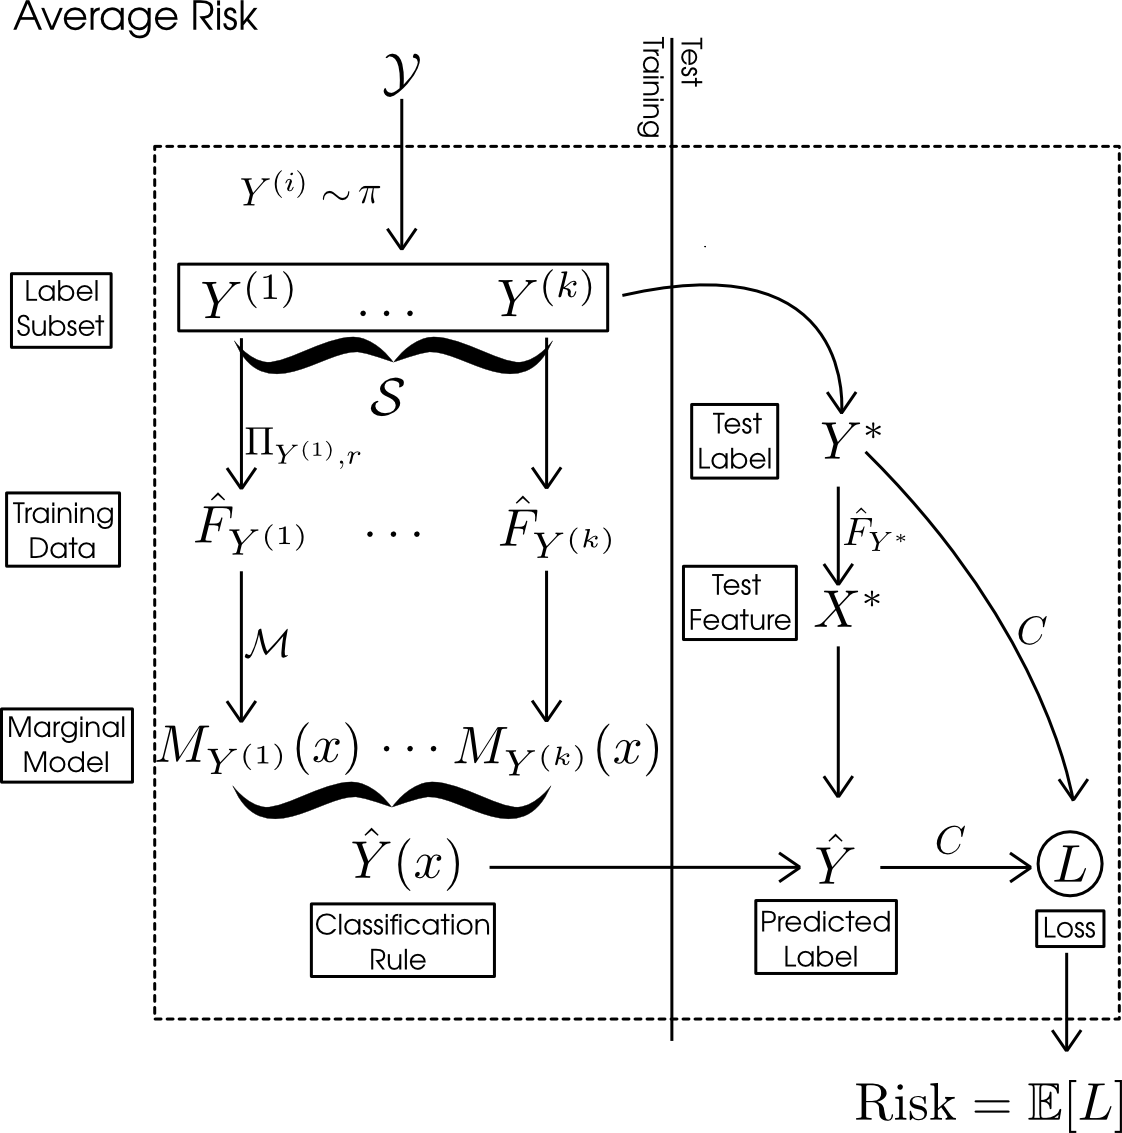
\includegraphics[scale = 0.3]{extrapolation_figures/average_risk.png}
\caption{Average risk}\label{fig:average_risk}
\end{figure}

%\subsection{Local polynomial regression}

%Explain background.

%Introduce the notation $\{(w_i, x_i, y_i)\}_{i=1}^n$: ordered triples
%of weight, predictor and response.



\section{Performance extrapolation for marginal classification models}
\label{sec:extrapolation}

Having outlined our assumption for randomized label subsets, the focus
of our theory moves towards understanding the $k$-class average risk:
that is, the expected risk of $\mathcal{F}$ when a random subset
$\mathcal{S}$ of size $k$ is drawn.

We obtain a method for estimating the risk in the second
classification task using data from the first.  The insight behind our
estimation method is obtained via an analysis of the average risk of
the classification task.

\subsection{Easy special cases}

Let us first mention two easy special cases, which can be handled
using existing machine learning methodology.

In the special case where $k_1 = k_2 = k$: that is, where the label
subsets $\mathcal{S}_1$ and $\mathcal{S}_2$ are the same size, it is
clear to see that any unbiased estimate of the risk of the classifier
$\mathcal{F}$ for the first classification problem is an unbiased
estimate of the average $k$-class risk.  Since various methods, such
as cross-validation can be used to obtain close-to-unbiased estimates
of the risk in a given classification problem, the problem is
essentially solved for this special case.

Meanwhile, in the case where $k_2 < k_1$, the problem can be solved by
repeatedly subsampling label sets of size $k_2$ from $\mathcal{S}_1$
and averaging unbiased estimates of the risk of each subsampled
classification task.  Aside from computational issues with respect to
computing or approximating the average of ${k_1}\choose{k_2}$
empirical accuracies, the problem is again more or less solved by
using existing methods.

Therefore, the challenging case is when $k_2 > k_1$: we want to
predict the performance of the classification model in a setting with
more labels than we currently see in the training set.

\subsection{Analysis of the average risk}

As we pointed out in the previous section, the challenging case for
the analysis is the ``undersampled'' regime where we wish to predict
the loss on a larger label set.  Given data with $k_1$ classes, we
already have means to estimate the average risk for all $k \leq k_1$,
so the challenge is to understand how the risk will ``extrapolate'' to
$k > k_1$.  Hence, the goal of the current analysis is to isolate the
effect of $k$, the size of the label subset, on the average risk.

Our strategy is to analyze the average risk \eqref{eq:avrisk_EL} by
means of \emph{conditioning on} the true label and its training
sample, $(y^*, \hat{F}_{y^*})$, and the test feature $x^*$
while \emph{averaging} over all the other random variables.  Define
the \emph{conditional average risk} $\text{CondRisk}_k((y^*, \hat{F}_{y^*}), x^*)$ as
\[
\text{CondRisk}_k((y^*, \hat{F}_{y^*}), x^*) = \E[L|Y^*=y^*, X^* = x^*, \hat{F}_{Y^*} = \hat{F}_{y^*}].
\]
Figure \ref{fig:conditional_risk} illustrates the variables which are
fixed under conditioning and the variables which are randomized.
Compare to figure \ref{fig:average_risk}.

Without loss of generality, we can write the label subset $\mathcal{S}
= \{Y^*, Y^{(1)},\hdots, Y^{(k-1)}\}$.  Note that due to independence,
$Y^{(1)},\hdots, Y^{(k-1)}$ are still i.i.d. from $\pi_0$ even
conditioning on $Y^* = y^*.$ Therefore, the conditional risk can be
obtained via the following alternative order of randomizations:
\begin{enumerate}
\item[C0.] 
Fix $y^*, \hat{F}_y^*,$ and $x^*$.  Note that $M_{y^*}(x^*)
= \mathcal{M}(\hat{F}_{y^*}; \pi(y^*))(x^*)$ is also fixed.
\item[C1.]
Draw the \emph{incorrect labels} $Y^{(1)},\hdots, Y^{(k)}$ i.i.d. from
$\nu$.  (Note that $Y^{(i)} \neq y^*$ with probability 1 due to the
continuity assumptions on $\mathcal{Y}$ and $\nu$.)
\item[C2.]
Draw the training samples for the incorrect labels
$\hat{F}_{Y^{(1)}},\hdots, \hat{F}_{Y^{(k-1)}}$.  This determines
\[
\hat{Y} = \argmax_{y \in \mathcal{S}} M_y(x^*)
\]
and hence
\[
L = C(\hat{Y}, y^*).
\]
\end{enumerate}
Compared to four randomization steps listed in
section \ref{sec:average_risk}, we have essentially conditioned on
steps A3 and A4 and randomized over steps A1 and A2.

%Let $G$ denote the joint distribution over $(X, Y)$ obtained by
%drawing $Y \sim \pi_0$ and $X \sim F_Y$.  Since $Y^*$ has the marginal
%distribution $\pi_0$, it follows that
%\begin{equation}\label{eq:rk_eq}
%\text{Average Risk}_k(\mathcal{F}) = \int \int R_k(y^*, x^*) dG(x^*, y^*).
%\end{equation}
%What we have done is to rewrite the average risk as the expectation of
%$R_k$, which depends on $k$, according to a measure $G$ which does
%\emph{not} depend on $k$.%

\begin{figure}[h]
\centering
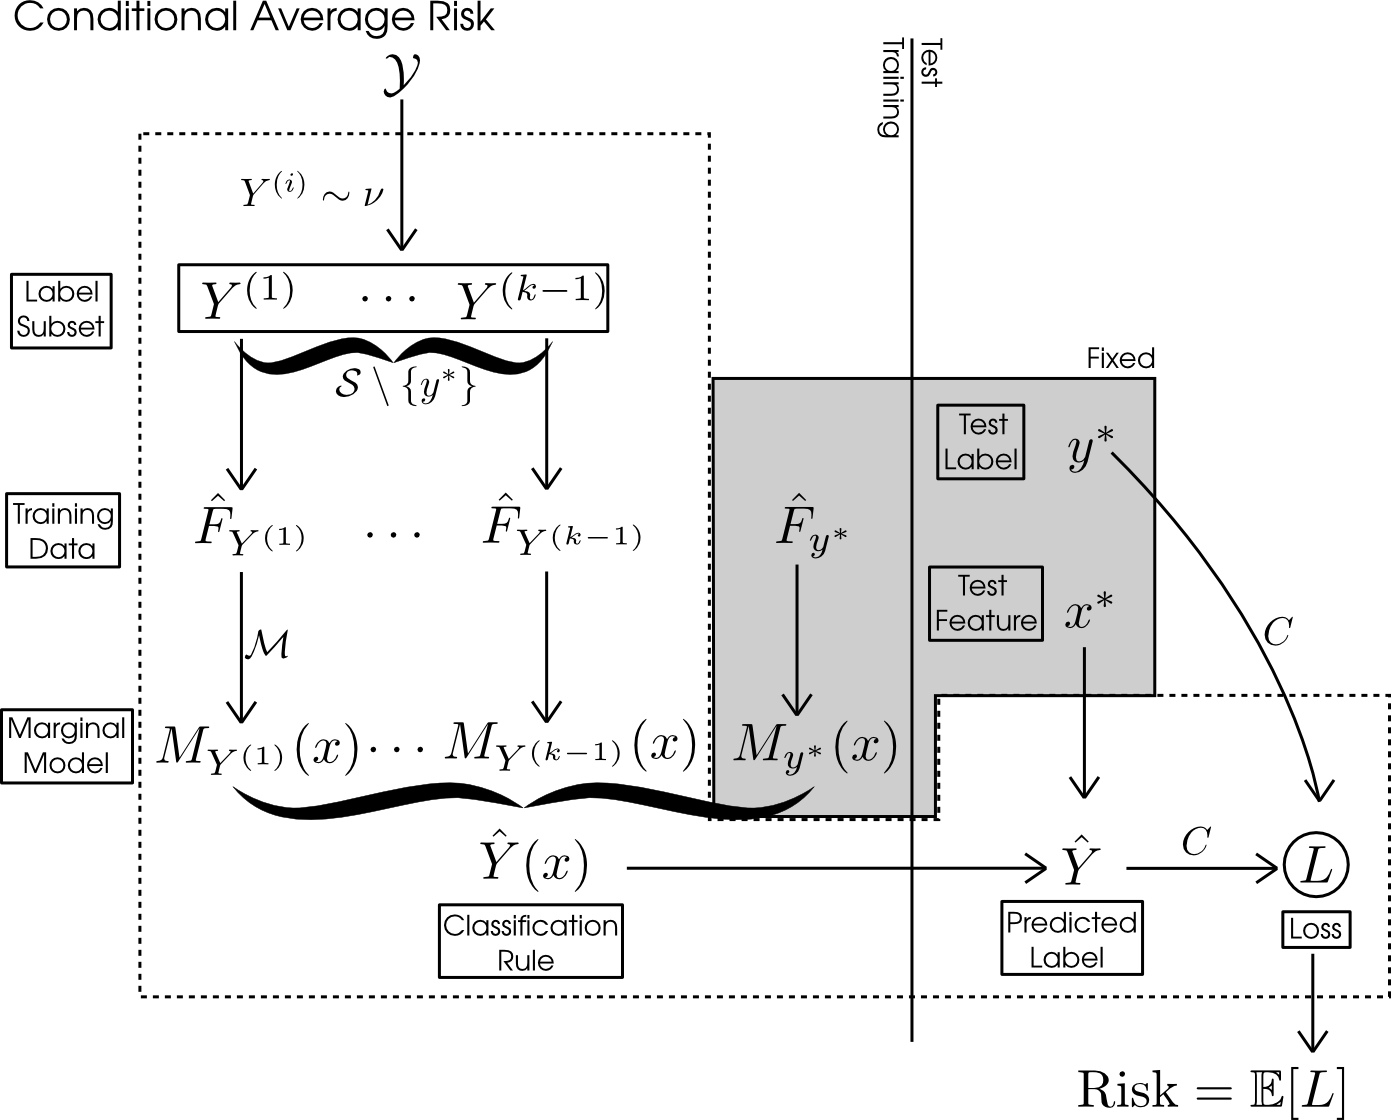
\includegraphics[scale = 0.3]{extrapolation_figures/conditional_risk.png}
\caption{Conditional average risk}\label{fig:conditional_risk}
\end{figure}

%However, we will further decompose $R_k$ into $k$-dependent and $k$-independent components.
Having defined the conditional average risk, we will now further
decompose it to expose its dependence on $k$.
We make the following additional technical assumptions:
\begin{itemize}
\item 
\emph{Scaling property of margins}: if $\mathcal{M}(\hat{F}_1, \pi_1)(x) >
\mathcal{M}(\hat{F}_2, \pi_2)(x)$ then also $\mathcal{M}(\hat{F}_1,
c\pi_1)(x) > \mathcal{M}(\hat{F}_2, c\pi_2)(x)$.
\item 
\emph{Tie-breaking condition}: for all $x \in \mathcal{X}$,
$\mathcal{M}(\hat{F}_Y, \pi_1)(x) = \mathcal{M}(\hat{F}_{Y'}, \pi_2)(x)$
with zero probability for $Y \neq Y'$ drawn from $\nu$.
\end{itemize}
The scaling property of margins is satisfied by most of the marginal
classifiers which are used in practice, and as such we do not consider
it to be a strong assumption.  Meanwhile, the tie-breaking condition
is a technical assumption which allows us to neglect the specification
of a tie-breaking rule in the case that margins are tied.  In
practice, one can simply break ties randomly, which is mathematically
equivalent to adding a small amount of random noise $\epsilon$ to the
function $\mathcal{M}$.

Now, in order to analyze the $k$-class behavior of the conditional
average risk, we begin by considering the \emph{two-class} situation.

In the two-class situation, we have a true label $y^*$ and one
incorrect label, $Y$.  Define the \emph{U-function}
$U_{x^*}(y^*, \hat{F}_{y^*})$ as the \emph{probability of correct
classification} in the two-class case.
The classification is correct if the margin
$M_{y^*}(x^*)$ is greater than the margin $M_Y(x^*)$, and incorrect
otherwise.  
Since we are fixing $x^*$ and $(y^*, \hat{F}_{y^*})$, the
probability of correct classification is obtained by taking an expectation:
\begin{align}\label{eq:U_function}
U_{x^*}(y^*, \hat{F}_{y^*}) &= \Pr[M_{y^*}(x^*) > \mathcal{M}(\hat{F}_Y, \pi_0(Y))(x^*)]
\\&= \int_{\mathcal{Y}} 
I\{
M_{y^*}(x^*) > \mathcal{M}(\hat{F}_{y}, \pi_0(y))(x)
\}
d\Pi_{y, r}(\hat{F}_y)
d\pi_0(y).
\end{align}
See also figure \ref{fig:U_function} for an graphical illustration of
the definition.

\begin{figure}[h]
\centering
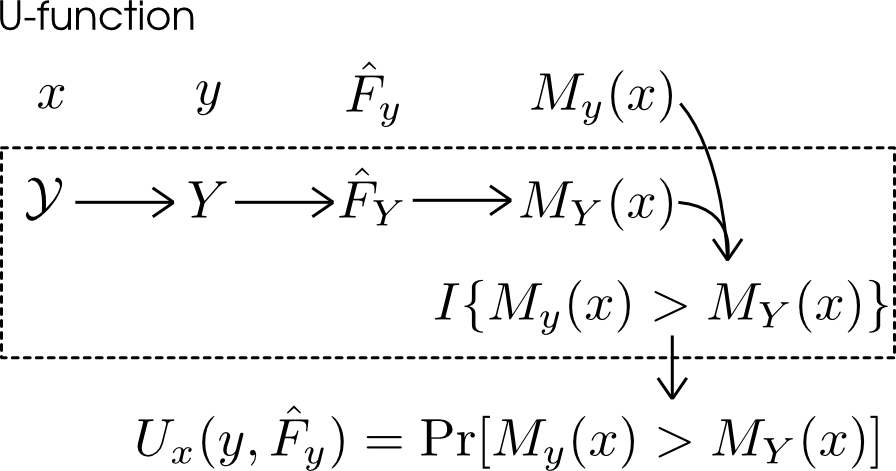
\includegraphics[scale = 0.4]{extrapolation_figures/U_function.png}
\caption{U-functions}\label{fig:U_function}
\end{figure}

An important property of the U-function, and the basis for its name,
is that the random variable $U_x(Y, \hat{F}_Y)$ for $Y \sim \nu$ and
$\hat{F}_Y \sim \Pi_{Y, r}$ is uniformly distributed for all
$x \in \mathcal{X}$.  This is proved in Lemma \ref{lemma:U_function}
in the appendix.

Now, we will see how the U-function allows us to understand the
$k$-class case.  Suppose we have true label $y^*$ and incorrect labels
$Y^{(1)},\hdots, Y^{(k-1)}$.  Note that the U-function
$U_{x^*}(y, \hat{F}_y)$ is monotonic in $M_y(x^*)$.  Therefore,
\[
\hat{Y} = \argmax_{y \in \mathcal{S}} M_y(x^*) = \argmax_{y \in \mathcal{S}} U_{x^*}(y, \hat{F}_y).
\]
Therefore, we have a correct classification if and only if the U-function value for the correct label
is greater than the maximum U-function values for the incorrect labels:
\[
\Pr[\hat{Y} = y^*] = \Pr[U_{x^*}(y^*, \hat{F}_{y^*}) > \max_{i=1}^{k-1} U_{x^*}(Y^{(i)}, \hat{F}_{Y^{(i)}})] =  \Pr[u^* > U_{max}].
\]
where $u^* = U_{x^*}(y^*, \hat{F}_{y^*})$ and $U_{max, k-1}
= \max_{i=1}^{k-1} U_{x^*}(Y^{(i)}, \hat{F}_{Y^{(i)}})$.  But now,
observe that we know the distribution of $U_{max, k-1}$!  Since
$U_{x^*}(Y^{(i)}, \hat{F}_{Y^{(i)}})$ are i.i.d. uniform, we know that
\begin{equation}\label{eq:umax_beta}
U_{max, k-1} \sim \text{Beta}(k-1, 1). 
\end{equation}
We now have the insights needed to analyze the simplest special case: zero-one loss.
\newline

\noindent \emph{Special case: 0-1 loss}.
For zero-one loss, which is $C(y, y') = I\{y = y'\}$, we have $L=1$ if
and only if $U_{max} > u^*$ and $L=0$ otherwise.  Therefore, the
conditional average risk is
\[
\text{CondRisk}_k((y^*, \hat{F}_{y^*}), x^*) = \Pr[U_{max} > u^*] = \int_{u^*}^1 (k-1) u^{k-2} du.
\]
Now the average risk can be obtained by integrating over the distribution of $U^* = U_{x^*}(y^*, \hat{F}_{y^*})$.
We have
\begin{align*}
\text{AvRisk}_k &= \E[ \int_{U^*}^1 (k-1) u^{k-2} du] 
\\&= \E[\int_0^1 I\{u \geq U^*\} (k-1) u^{k-2} du ]
\\&= (k-1) \int_0^1 \Pr[U^* \leq u] u^{k-2} du.
\end{align*}
Or equivalently,
\[
\text{AvRisk}_{k, r, \nu}((y^*, \hat{F}_{y^*}), x^*) = (k-1) \int \bar{K}(u) u^{k-2} du.
\]
where $\bar{K}(u)$ denote the cumulative distribution function of $U^*$ on $[0,1]$:
\[
\bar{K}(u) = \Pr[U_{x^*}(y^*, \hat{F}_{y^*}) \leq u].
\]
We have expressed the average risk expressed as a weighted integral of
a certain function $\bar{K}(u)$ defined on $u \in [0,1]$.  We have
clearly isolated the part of the average risk which is independent of
$k$--the univariate function $\bar{K}(u)$, and the part which is
dependent on $k$--which is the density of $U_{max}$.

In section \ref{sec:estimation}, we will develop estimators of
$\bar{K}(u)$ in order to estimate the $k$-class average risk.
But now let us return to the general case.
\newline

\noindent \emph{General loss functions.}
The case for general cost functions is somewhat more complicated,
since knowledge of $U_{max}$ is not sufficient to determine $L$.  In
short, this is because $U_{max}$ by itself is insufficient to
determine $\hat{Y}$, and therefore $L=C(\hat{Y}, y^*)$.  However, we
can resolve this issue by noting that for the purposes of computing
the expected loss, it suffices to have the \emph{conditional
distribution} of $\hat{Y}$ given $U_{max}$.  Even though $U_{max}$
does not deterministically map onto a unique $\hat{Y}$, it determines
a conditional distribution of $\hat{Y}$ which allows us to compute
$\E[L|U_{max}, x^*, y^*, \hat{F}_{y^*}]$.

Now, a key fact is that the conditional distribution of $\hat{Y}$
given $U_{max}$ \emph{does not depend} on $k$.  To see this fact,
suppose without loss of generality that $\hat{Y} = Y^{(k-1)}.$ Then
the joint density of $Y^{(1)},\hdots, Y^{(k-1)}$ given $U_{max} =
u$ can be written
\[
p(y^{(1)},\hdots, y^{(k-1)}) \propto 
\nu(y^{(k-1)})\frac{d}{dt}\Pr[U_{x^*}(y^{(k-1)}, \hat{F}_{y^{(k-1)}}) \leq t]|_{t=u}
\prod_{i=1}^{k-2}\nu(y^{(i)})\Pr[U_{x^*}(y^{(k-1)}, \hat{F}_{y^{(k-1)}}) < u].
\}
\]
up to a normalizing constant.  Note that the term
$\frac{d}{dt}\Pr[U_{x^*}(y^{(k-1)}, \hat{F}_{y^{(k-1)}}) \leq t]$ is the
density of the random variable
$U_{x^*}(Y^{(k-1)}, \hat{F}_{Y^{(k-1)}})$. From the density, we can see
that $Y^{(1)},\hdots, Y^{(k-1)}$ are conditionally independent given
$U_{max} = u$, hence the marginal density of $\hat{Y}=Y^{(k-1)}$ can
be written
\[
p(\hat{y}) \propto \nu(\hat{y})\frac{d}{dt}\Pr[U_{x^*}(y^{(k-1)}, \hat{F}_{y^{(k-1)}}) \leq t]|_{t=u}.
\]

The only property of the conditional distribution of $\hat{Y}|U_{max} = u$ that is needed is
the expectation of $L = C(\hat{Y}, y^*)$.  Therefore, define the \emph{conditional expected loss} $K((y^*, \hat{F}_{y^*}), x^*, u)$ by
\begin{equation}\label{eq:Kfunc}
K((y^*, \hat{F}_{y^*}), x^*, u) = \begin{cases} 0 \text{ if } u < u^*\\
\E[C(\hat{Y}, y^*)|U_{max} = u, x^*, y^*, \hat{F}_{y^*}] \text{ otherwise.}
\end{cases}
\end{equation}
We have the two cases $u < u^*$ and $u > u^*$ since when $U_{max} <
u^*$, the correct label is chosen and the loss is zero.  Otherwise, an
incorrect label is chosen, and the expected loss must be calculated
using the conditional distribution of $\hat{Y}$.

Again, since the conditional distribution of $\hat{Y}|U_{max}, x^*,
(y^*, \hat{F}_{y^*})$ is independent of $k$, the conditional cost
function is also independent of $k$.

With the conditional cost function and the distribution of $U_{max}$ both in hand, we can compute the average conditional risk
\[
\text{CondRisk}_k((y^*, \hat{F}_{y^*}), x^*) = (k-1) \int K((y^*,\hat{F}_{y^*}), x^*, u) u^{k-2} du.
\]
Now the average risk can be obtained by integrating over $(Y^*, \hat{F}_{Y^*}),$ and $X^*$.
\[
\text{AvRisk}_{k, r, \nu}((y^*, \hat{F}_{y^*}), x^*) = (k-1) \int \bar{K}(u) u^{k-2} du.
\]
where
\begin{equation}\label{eq:Kbar}
\bar{K}(u) = \int K((y^*,\hat{F}_{y^*}), x^*, u) \nu(y^*)dy dF_{y^*}(x^*) d\Pi_{y^*, r}(\hat{F}_{y^*}).
\end{equation}


This is the key result behind our estimation method, and we restate it
in the following theorem.

\begin{theorem}\label{theorem:avrisk_identity}
Suppose $\pi_0$, $\{F_y\}_{y \in \mathcal{Y}}$ and marginal classifier
$\mathcal{F}$ satisfy the marginal scaling condition tie-breaking
condition.  Then, under the
definitions \eqref{eq:U_function}, \eqref{eq:Kfunc},
and \eqref{eq:Kbar}, we have
\begin{equation}\label{eq:avrisk_identity}
\text{AvRisk}_{k, r, \nu}((y^*, \hat{F}_{y^*}), x^*) = (k-1) \int \bar{K}(u) u^{k-2} du.
\end{equation}
\end{theorem}

The proof is given in the appendix.

Having this theoretical result allows us to understand how the
expected $k$-class risk scales with $k$ in problems where all the
relevant densities are known.  However, applying this result in
practice to estimate $\text{Average Risk}_k$ requires some means of
estimating the unknown function $\bar{K}$--which we discuss in the
following.

\subsection{Estimation in the general case}\label{sec:estimation}

Now we address the problem of estimating $\text{AvRisk}_{k_2,
r_{train}}$ from data.  As we have seen from
Theorem \ref{theorem:avrisk_identity}, the $k$-class average risk of
a marginal classifier $\mathcal{M}$ is a functional of a object called
$\bar{K}(u),$ which depends marginal model $\mathcal{M}$ of the
classifier, the joint distribution of labels $Y$ and features $X$ when
$Y$ is drawn from the sampling density $\nu$.

Therefore, the strategy we take is to attempt to estimate $\bar{K}$
for then given classification model, and then plug in our estimate of
$\bar{K}$ into the integral \eqref{eq:avrisk_identity} to obtain an
estimate of $\text{AvRisk}_{k_2, r_{train}}$.  Having decided to
estimate $\bar{K}$, there is then the question of what kind of model
we should assume for $\bar{K}$.  While a nonparametric approach may be
ideal, for the case of general loss functions we will adopt a
parametric model: that is the subject of this section.  On the other
hand, for the special case of zero-one loss
(Section \ref{sec:sp_case}), we take a nonparametric approach.

Even restricting ourselves to parametric models, there are wide
variety of parametric families one might consider for $\bar{K}(u)$.
As it turns out, the $d$-th order polynomial model is unique for
enabling unbiased estimation of the average risk.  Therefore, let us
assume
\[
\bar{K}(u) = \sum_{\ell = 0}^d \beta_\ell u^\ell.
\]

Recall that the data consists of $k_1 < k_2$ classes, $\mathcal{S}_1 =
\{y^{(1)},\hdots, y^{(k_1)}\}$. For each $y^{(i)}$ we have training sample $\hat{F}_{y^{(i)}}$, and
$r_{test}$ test repeats per class, $(x_1^{(i)},\hdots,
x_{r_{test}}^{(i)})$.

The marginal model $\mathcal{M}$ yields margins for each point in the
test set for each label in $\mathcal{S}_1$.  Define the margins
\[
M_{i, j, \ell} = \mathcal{M}(\hat{F}_{y^{(\ell)}}; \pi_1(y^{(\ell)}))(x_j^{(i)}).
\]
The predicted label for each test point is
\[
\hat{y}_{i,j} = y^{(\argmax_{\ell \in \{1,\hdots, k\}} M_{i, j, \ell})}.
\]
Therefore, an unbiased estimate of the risk (which is also an unbiased
estimate of the $k_1$-class average risk) is
\[
\text{Test Risk} = \frac{1}{r_{test}}\sum_{i=1}^k \sum_{j=1}^{r_{test}} C(\hat{y}_{i, j}, y^{(i)}).
\]

Now we turn to the question of estimating the function $\bar{K}(u)$.
Suppose that hypothetically, we could have observed the quantities
$U_{i, j, \ell}$, defined
\[
U_{i, j, \ell} = U_{x_j^{(i)}}(y^{(\ell)}, \hat{F}_{y^{(\ell)}}).
\]
for $i \neq \ell = 1,\hdots, k_1$, and $j = 1,\hdots, r_{test}$.
Also define
\[
C_{i,j, \ell} = C(y^{(\ell)}, y^{(i)})I\{M_{i, j, \ell} > M_{i, j, i}\}
\]
for $i \neq \ell = 1,\hdots, k_1$, and $j = 1,\hdots, r_{test}$.
By definition, we have
\[
\bar{K}(u) = \E[C(Y, Y^*)I\{U_{X^*}(Y) > U_{X^*}(Y^*)\}] = \E[C_{i,\ell} | U_{i, j, \ell} = u].
\]
This means that $\bar{K}(u)$ could be estimated via a $d$-th order polynomial regression
\[
\hat{\beta} = \argmin_{\beta} \sum_{i\neq \ell=1, j = 1}^{k_1, r_{test}} \left(C_{i,j,\ell} - \sum_{h=0}^d \beta_h U_{i,j, \ell}^h\right)^2.
\]
However, this is not possible in
practice because $U_{i,j,\ell}$ are not directly observed.

Instead, we have an unbiased estimates of $\hat{U}_{i, j, \ell}$ via
\[
\hat{U}_{i,j, \ell}^{(1)} = \frac{1}{(k_1-2)}\sum_{m \neq i \neq \ell} I\{M_{i, j, \ell} > M_{i, j, m}\}
\]
Since we have \emph{errors-in-covariates}, it is necessary to make use
of the \emph{covariate adjustment} technique (see
Appendix \ref{sec:me}).  Covariate adjustment is justified since the
measurement error in $\hat{U}_{i,j, \ell}$ is independent of the
response given the true covariates:
\[
\hat{U}_{i,j,\ell} \perp C_{i,j,\ell} | U_{i, j,\ell}.
\]
Covariate adjustment in this case amounts to obtaining unbiased estimates of
the powers $U_{i,j,\ell}^h$.

% reconfigure notation to get rid of indicators somehow??
There exist U-statistic estimators of the higher powers of
$\hat{U}_{i,j,\ell}^h$.  For instance, for $h=2$, the estimator is
\[
\hat{U}_{i,j,\ell}^{(2)} = \frac{1}{ (k_1-2)(k_1-3) } \sum_{m_1\neq m_2 \neq i \neq \ell} I\{M_{i, j, \ell} > M_{i, j, m_1}\} I\{M_{i, j, \ell} > M_{i, j, m_2}\}.
\]
In general, the U-statistic is
\[
\hat{U}_{i, j, \ell}^{(h)} = \frac{(k_1-h-2)!}{(k_1-2)!} \sum_{m_1 \neq \cdots \neq m_h \neq i \neq \ell} \prod_{z=1}^h I\{M_{i, j, \ell} > M_{i, j, m_z}\}.
\]
The U-statistic estimator works because $M_{i, j}^m$ are conditionally
independent given $x^{(i)}_j$, $y^{(i)}$, and $y^{(\ell)}$ for $m
= \{1,\hdots, k_1\}\setminus \{i, \ell\}$.

Then, define
\[
\hat{\beta} = \argmin_\beta \sum_{i\neq \ell=1, j = 1}^{k_1, r_{test}} \left(C_{i,j,\ell} - \sum_{h=0}^d \beta_h \hat{U}_{i,j, \ell}^{(h)}\right)^2.
\]
By the properties of covariate adjustment (Appendix \ref{sec:me},) $\hat{\beta}$ is an unbiased estimate of $\beta$.
Therefore we obtain the estimate
\[
\hat{K}(u) = \sum_{\ell = 0}^d \hat{\beta}_\ell u^\ell.
\]

Now in order to predict the average risk for $k_2$ classes, we use \eqref{eq:avrisk_identity} and compute
\begin{align*}
\widehat{\text{AvRisk}_k} &= (k-1) \int_0^1 \hat{K}(u) u^{k-2} du
\\&= (k-1) \int_0^1 \sum_{\ell = 0}^d \hat{\beta}_\ell u^\ell u^{k-2} du
\\&= (k-1) \sum_{\ell = 0}^d \hat{\beta}_\ell  \int_0^1 u^{\ell + k-2} du
\\&= (k-1) \sum_{\ell = 0}^d \frac{\hat{\beta}_\ell}{\ell + k - 1}.
\end{align*}
Again, since $\hat{\beta}$ is unbiased for $\beta$, it follows that
$\widehat{\text{AvRisk}_{k_2}}$ is an unbiased estimator for the
average risk $\text{AvRisk}_{k_2}$.

The algorithm is summarized below.

\fbox{
  \parbox{\textwidth}{
    \textbf{Estimation of average risk under $d$th order polynomial model}

    \emph{Inputs:}
    \begin{itemize}
    \item Marginal model $\mathcal{M}$ and cost function $C$.
    \item Class labels $y^{(i)}$ and prior weights $\pi_1(y^{(i)})$ for $i = 1,\hdots, k_1$.
    \item Training sample $\hat{F}_{y^{(i)}}$ and test sample $(x_1^{(i)},\hdots, x_{r_{test}}^{(i)})$ for $i = 1,\hdots, k_1$.
    \end{itemize}

    \emph{Parameters:}
    \begin{itemize}
    \item $k_2$: specifies number of classes for the estimation target $\text{AvRisk}_{k_2}$.
    \item $d$: order of the polynomial model assumed for $\bar{K}(u)$.
    \end{itemize}

    \emph{Algorithm:}
    \begin{enumerate}
    \item For $i = 1,\hdots, k_1$, $j= 1,\hdots, r_{test}$, and $\ell = 1,\hdots, k_1$, compute
    \[
    M_{i, j, \ell} = \mathcal{M}(\hat{F}_{y^{(\ell)}}; \pi_1(y^{(\ell)}))(x_j^{(i)}).
    \]
    and
    \[
    C_{i,j, \ell} = C(y^{(\ell)}, y^{(i)})I\{M_{i, j, \ell} > M_{i, j, i}\}.
    \]
    \item  For $i\neq \ell = 1,\hdots, k_1$, $j= 1,\hdots, r_{test}$, and $h = 0,\hdots, d$, compute
    \[
    \hat{U}_{i, j, \ell}^{(h)} = \frac{(k_1-h-2)!}{(k_1-2)!} \sum_{m_1 \neq \cdots \neq m_h \neq i \neq \ell} \prod_{z=1}^h I\{M_{i, j, \ell} > M_{i, j, m_z}\}.
    \]
    \item Find the least-squares solution
    \[
    \hat{\beta} = \argmin_\beta \sum_{i\neq \ell=1, j = 1}^{k_1, r_{test}} \left(C_{i,j,\ell} - \sum_{h=0}^d \beta_h \hat{U}_{i,j, \ell}^{(h)}\right)^2.
    \]
    \item Output
    \[
    \widehat{\text{AvRisk}_{k_2}} = (k_2-1) \sum_{\ell = 0}^d \frac{\hat{\beta}_\ell}{\ell + k_2 - 1}.
    \]
    \end{enumerate}
  }
}
% summary of algorithm


\subsection{Convergence analysis}



Taking a fairly conservative analysis, we will use the universal variance bound
\[
\Var[\bar{C}_m] \leq \frac{1}{4r}
\]
which holds given the condition $\sup_{\mathcal{Y}^2} C(y, y') \leq 1.$

We have the explicit formulas
\[
W_\ell = \frac{\ell!(K-\ell)!}{K!}
\]
and
\[
Z_{m, \ell} = \frac{(m+\ell-1)!(k-1)!}{(m-1)!(k+\ell-1)!}.
\]

The variance of the unbiased estimate of average risk is bounded by
\[
\Var[\widehat{AvRisk}_k(\mathcal{F})] \leq \frac{1}{4r} \vec{W}^T (\bZ^T \bZ)^{-1} \vec{W}.
\]
The bound depends only on the quantities $r, d, k, K$, and can be
easily computed numerically.  However, it is easy to see that in the
$r \to \infty$ limit, consistent estimation results.  It remains to
understand how the asymptotic performance of our estimation procedure
depends on the parameters $d, k, K$.

Define
\[
\kappa(k, K, d) = \vec{W}^T (\bZ^T \bZ)^{-1} \vec{W}.
\]


\subsection{Monotonicity assumption}

Assuming that $\bar{K}(u)$ in monotone in $u \in [0,1]$.
Justification and implications.

\section{Special case: uniform prior and zero-one loss}\label{sec:sp_case}

For the special case of zero-one loss and uniform prior, the theory
becomes simplified and additional methods of estimation are possible.

Define
\[
\gamma_m = \int_0^1 \bar{K}(u)  \frac{k_1!}{(m-1)!(k_1-m)!} u^{m-1} (1-u)^{k_1-m} du
\]
for $m = 1,\hdots, k_1$.

Define the \emph{ranks}
\[
R_{i, j, \ell} = (k-1)\hat{U}_{i, j, \ell}.
\]
Due to the uniform prior, $R_{ij}^\ell \in \{0,\hdots, k_1-1\}$.

Define
\[
C_{ij}^{(h)} = \sum_{\ell=1}^k I\{R_{i, j, \ell} = h - 1\} C_{i, \ell},
\]
i.e., the cost incurred for the class with the $h$th smallest rank for
the observation $x_i^{(\ell)}$.

Note that the test risk for $k_1$ classes can be written as
\[
\text{Test Risk}_k = \frac{1}{r_{test}k_1}\sum_{i=1,j=1}^{k_1,r_{test}} C_{ij}^{(k_1)}.
\]

Since $C_{ij}^\ell$ is now a binary random variable, we have
\[
C_{ij}^{(h)} \sim \text{Bernoulli}(\gamma_h).
\]

If $C_{ij}^{(h)}$ were independent, one could estimate $\gamma_h$ by
maximizing the log-likelihood
\begin{equation}\label{eq:pseudolikelihood1}
\mathcal{L}(\vec{\gamma}) = \sum_{i=1,j=1,h=1}^{k_1, r_{test}, k_1} C_{ij}^{(h)} \log \gamma_h + (1-C_{ij})^{(h)} \log (1-\gamma_h)
\end{equation}

However, since $C_{ij}^{(h)}$ are not independent, the equation
\eqref{eq:pseudolikelihood1} is not a likelihood, but a
\emph{pseudolikelihood}.  Nevertheless, one can attempt to estimate
$\gamma_h$ using the method.

The basic idea of using pseudolikelihood leads to many different
practical approaches for estimating the average $k$-class risk.  We tried the following approaches:
\begin{enumerate}
\item Estimate unconstrained $\gamma_h$, then find a function
  $\bar{K}(u)$ which satisfies the moment constraints implied by the
  estimates $\hat{\gamma}_h$.  Estimate $\text{AvgRisk}_k$ by plugging
  in the estimated $\hat{K}(u)$ into \eqref{eq:avrisk_identity}.
\item Let $\hat{K}(u)$ be constrained by the test risk (which is unbiased for the $k_1$-class average risk,)
\[
\text{Test Risk}_l = \int_0^1 \hat{K}(u) k_1 u^{k_1 -1} du.
\]
Under this moment constraint, estimate $\hat{K}(u)$ using pseudolikelihood.
%needs to be clarified how pseudolikelihood can be used to estimate either hatKu or gamma
\item Either of the above two approaches, plus a monotonicity constraint on $\hat{K}(u).$
\end{enumerate}







\appendix
\section{Appendix}
\subsection{Measurement error models}\label{sec:me}

We make use of measurement error regression models in
section \ref{sec:estimation}: in particular, the regression adjustment
method.  In this section we focus on the specific measurement error
models and methods that are used in this work: for an overview of the
subject, the reader can consult (Caroll, 2005).

In the traditional setting of linear regression, one observes data
$(\bx_i, y_i)_{i=1}^n$ where the data is generated from the linear model
\[
Y_i = \bx_i^T \beta + \epsilon_i
\]
for some random noise variables $\epsilon_i$ that satisfy
$\E[\epsilon_i] = 0$.  However, in measurement error models, we assume
that $\bX_i$ is not directly observed.  (We write $\bX_i$ instead of
$\bx_i$, since in some measurement error models the true covariates
are also assumed to be random.)  Instead, one only has access to a
corrupted version of the covariates, $\bZ_i$.  We say that $\bZ_i$
are \emph{noisy measurements} of $\bX_i$.  Depending on the noise
model for $\bZ_i|\bX_i$, the OLS coefficients for the regression of
$Y$ on $\bZ$
\begin{equation}\label{eq:ols}
\hat{\beta}_{naive} = \argmin_\beta \sum_{i=1}^n (y_i - \bz_i^T \beta)^2
\end{equation}
may be a biased estimated of $\beta.$

Suppose we can true the true covariates $\bX_i$ as random variables.
We say that the measurement error is \emph{nondifferential} if $\bZ_i$
is conditionally independent of $Y_i$ given $\bX_i$.  In other words,
the distribution of $Y$ only depends on $(\bX, \bZ)$ through $\bX$.
For nondifferential measurement error, it is possible to obtain an
unbiased estimate of $\beta$ by using \emph{regression calibration}.

Regression calibration requires the ability to estimate or exactly
compute the conditional expectation $\E[\bX_i|\bZ_i].$ For simplicity,
suppose that there exists a known function $g$ such that $g(\bz)
= \E[\bX|\bZ = \bz].$ Then, define $\hat{\bx}_i = g(\bz_i)$ for $i =
1,\hdots, n$.  The calibrated estimate of $\beta$ is
\begin{equation}\label{eq:rc}
\hat{\beta}_{rc} = \argmin_\beta \sum_{i=1}^n (y_i - \hat{\bx}_i^T \beta)^2
\end{equation}
We can see that the estimate is unbiased by the following identity.
Observe that
\begin{align*}
\E[Y|\hat{\bX}] &= \E[Y|\bZ]
\\&= \E[\bX^T \beta + \epsilon|\bZ]
\\&= \E[\bX|\bZ]^T \beta
\\&= \hat{\bX}^T \beta.
\end{align*}
This identity shows that $\beta$ is the population regression
coefficient of $Y$ on $\hat{\bX}.$ Therefore, applying ordinary least
squares to the data $(\hat{\bx}_i, y_i)$ will produce an unbiased
estimate of the population regression coefficient--that is, $\beta.$

In the \emph{Berkson} measurement error model, we have
\[
\bx_i = \bz_i + \eta_i
\]
where $\eta_i$ are independent error variates such that
$\eta_i \perp \epsilon_i | \bz_i.$ Thus, in the Berkson model, the
measurement error is nondifferentiable, and regression calibration can
be applied to estimate $\beta$.  Furthermore, supposing that
$\E[\eta_i]=0$, then we can simply take $\hat{\bx} = \bz_i$--in other
words, the naive OLS estimate is equivalent to the regression
calibration estimate, and therefore no correction is needed.
However, suppose we have a \emph{nonlinear additive model} of the form
\[
Y_i = \sum_{j=1}^d \beta_j h_j(X_i) + \epsilon_i.
\]
Then, even if $\E[X_i|Z_i] = Z_i$, it is not true in general that
$\E[h_j(X_i)|Z_i] = Z_i$.  Therefore, one needs to construct unbiased
(or approximately unbiased) estimates $H_{i,j}$ such that
\[
\E[H_{i,j}|Z_i] = \E[h_j(X_i)|Z_i]
\]
and estimate $\beta$ via
\[
\hat{\beta}_{rc} = \argmin_\beta \sum_{i=1}^n \left(y_i - \sum_{j=1}^d \beta_j H_{i, j} \right)^2.
\]

\subsection{Regression with importance sampling}

This section describes a fairly specialized problem in linear
regression which we encounter in section \ref{sec:estimation}.

Suppose $\{F_\theta\}$ is a family of bivariate distributions for
random variates $(\bX, Y)$, with $\bX \in \mathbb{R}^p$ and
$Y \in \mathbb{R}$, indexed by parameter $\theta \in \Theta.$ Let $G$,
$H$ be distributions on $\Theta$.  Define $F^*$ as the bivariate
distribution obtained by mixing over $\theta \sim G$:
\[
F^*(A) = \int_\Theta F_\theta(A) dG(\theta)
\]
for any measurable set $A \in \mathbb{R}^p \times \mathbb{R}$.  Now
suppose that $Y$ has a conditional expectation which is linear in
$\bX$ under $F^*$:
\[
\E_{F^*}[Y|\bX] = \bX^T \beta
\]
for some $\beta \in \mathbb{R}^p$.
Equivalently,
\[
\int_{A \times \mathbb{R}} y I(\bx \in A) dF^*(\bx, y) = \beta^T \left(\int_{A \times \mathbb{R}} \bx I(\bx \in A) dF^*(\bx, y)\right)
\]
for all measurable $A \subset \mathbb{R}^p$.

However, the conditional expectation $\E_{F_\theta}[Y|\bX]$ need not
be linear in $\bX$ for $\theta \in \Theta$.

Now, suppose we observe data
triples $(\theta_i, x_i, y_i)$ which are generated as follows:
\begin{itemize}
\item Draw $\theta_i \sim H$.
\item Draw $(X_i, Y_i) \sim F_\theta$.
\end{itemize}
Let $\eta$ be a Radon-Nikodym derivative of $H$ with respect to $G$, so that $H = \eta G$.
Then an unbiased estimate of $\beta$ can be obtained via an importance sampling estimate:
\[
\hat{\beta} = \argmin_\beta \sum_{i=1}^n \frac{1}{\eta(\theta_i)} (y_i - \bx_i^T \beta).
\]

\subsection{Proofs}

\begin{lemma}\label{lemma:U_function}
Defining $U_{y,\hat{F}_y}(x)$ as in \eqref{eq:U_function}.
\end{lemma}



\section*{References}

\small

[1] Kay, K. N., Naselaris, T., Prenger, R. J., \& Gallant, J. L. (2008). ``Identifying natural images from human brain activity.'' 
\emph{Nature}, 452(March), 352-355.

[2] Deng, J., Berg, A. C., Li, K., \& Fei-Fei, L. (2010). ``What does classifying more than 10,000 image categories tell us?'' \emph{Lecture Notes in Computer Science}, 6315 LNCS(PART 5), 71-84. 

[3] Garfield, S., Stefan W., \& Devlin, S. (2005). ``Spoken language classification using hybrid classifier combination." 
\emph{International Journal of Hybrid Intelligent Systems} 2.1: 13-33.

[4] Anonymous, A. (2016). ``Estimating mutual information in high dimensions via classification error.''  Submitted to 
\emph{NIPS 2016.}

[5] Tewari, A., \& Bartlett, P. L. (2007). ``On the Consistency of Multiclass Classification Methods.''
\emph{Journal of Machine Learning Research}, 8, 1007-1025.

[6] Hastie, T., Tibshirani, R., \& Friedman, J., (2008). \emph{The elements
of statistical learning.} Vol. 1. Springer, Berlin: Springer series in
statistics.

[7] Arnold, Barry C., \& Strauss, D.  (1991). ``Pseudolikelihood estimation: some examples." \emph{Sankhya: The Indian Journal of Statistics, Series B}: 233-243.

[8] Cox, D.R., \& Hinkley, D.V. (1974). \emph{Theoretical statistics.} Chapman and Hall. ISBN 0-412-12420-3

[9] Lawson, C. L., \& Hanson, R. J. (1974). \emph{Solving least squares problems.} Vol. 161. Englewood Cliffs, NJ: Prentice-hall.

[10] Hong, J., Mohan, K. \& Zeng, D. (2014). ``CVX. jl: A Convex Modeling Environment in Julia."

[11] Domahidi, A., Chu, E., \& Boyd, S. (2013). "ECOS: An SOCP solver for embedded systems." \emph{Control Conference (ECC), 2013 European. IEEE.}

[12] Achanta, R., \& Hastie, T. (2015) "Telugu OCR Framework using Deep Learning." arXiv preprint arXiv:1509.05962 .


\end{document}






















